\chapter{PROPOSED SOLUTION}
\label{chap:solution}

This chapter describes the proposed solution which is a system consists of two subsystems: A crowd-sourcing system and an analysis system. In \textit{Requirement analysis and System overview} subsection, everything is briefly described as a whole. In two last sections, structure and details of two subsystems are defined more comprehensively.

\section{Requirement analysis and system overview}
\subsection{Requirement analysis}

To be able to utilize data to serve a security purpose, the most obvious method would be to analyze visual data such as photos and videos, and the current most effective way to do so is using Artificial Intelligence. In recent years, advancements in Artificial Intelligence, especially in Neural Networks, significantly enhanced the development of computer vision field. On the famous ImageNet \footnote{Source: \url:{http://www.image-net.org/challenges/LSVRC/}} dataset, trained neural networks can now generate results that are better than human in classifying images (Figure \ref{chap3:deeplearning_vs_human}). 
For Deep learning models to be successful, sufficient training data must be provided. \cite{DBLP:journals/corr/SunSSG17} found out that the effectiveness of computer vision related tasks scales logarithmically with the amount of training data. Regardless of the importance of data in Deep learning models, there are few to none security datasets that are suitable for the environment of Vietnam.  \\

\begin{center}
    \begin{figure}[H]
    \centering
    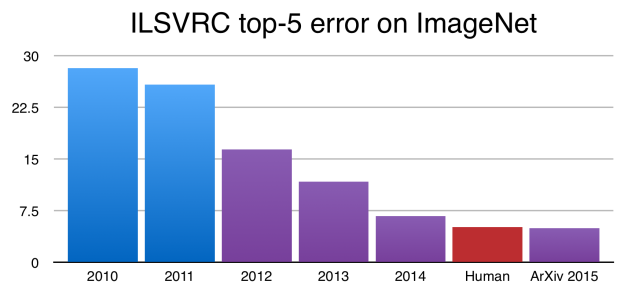
\includegraphics[width=0.75\columnwidth]{images/chap3/deeplearning_vs_human.png}
    \footcaption{Neural Network out-performing human in 2015 on ImageNet Large Scale Visual Recognition Challenge}
    \label{chap3:deeplearning_vs_human}
    \end{figure}
\end{center}

\footnotetext{Source: \url:{ https://devblogs.nvidia.com/mocha-jl-deep-learning-julia/}}

A traditional method of collecting data would be to set up an array of cameras at desired locations and then obtain their recordings. Those recording would later be labeled by specialists and processed to form a dataset. This way of doing is expensive and require a lot of human resources.
One other method of data collection is to implement Web crawler to pull data from the internet automatically. This method would be most useful for getting a large amount of data given a keyword. Data achieved by this method often contain considerable noise. In the context of security, those data would not be suitable because they are incredibly diverse and do not fit the Vietnamese environment.
Crowdsourcing is one of the effective methods of data collection. The idea behind crowdsourcing is to build datasets with the help of a large group of people. An example of this kind of model is Wikipedia \footnotetext{Source: \url:{https://www.wikipedia.org}}
. Wikipedia is an enormous web-based, collaborative encyclopedia which has over 100,000 volunteers contributing new information to the system daily. The success of Wikipedia proves that people gladly contribute to a system without profit if it brings a greater good. \\
But how can people be encouraged to contribute their knowledge and information? Through interaction with others had been proven successful in increasing engagement. Social media has been a popular trend among Vietnamese people. Therefore, this thesis proposes building a social media platform for security. This social media serves as a point of interaction with users, as well as allow people to contribute their knowledge to the system. \\
Figure \ref{chap3:system_overview_basic} shows a concise overview of how the system operates. Users interact with the \textbf{Crowd-sourcing system} through \textbf{User Interfaces}. The input of users can come in the form of images, videos or label contribution and are stored in the database. The system is also responsible for obtaining appropriate contents from the database to display to users through user interfaces.
\begin{center}
    \begin{figure}[H]
    \centering
    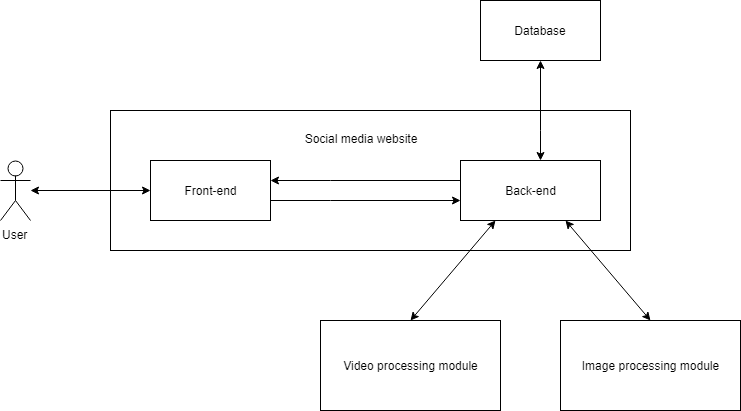
\includegraphics[width=1\columnwidth]{images/chap3/system_overview_basic.png}
    \caption{An overview of the system}
    \label{chap3:system_overview_basic}
    \end{figure}
\end{center}
Whenever there is a video to analyze,the server will send it to the \textbf{Video classifier module}, then get the results back. Results returned from video classifier module are classified activity from the video and frames that contain faces in them. \textbf{Face Recognition module} does the job of identifying people in images. Results of both \textbf{Video classifier module} and \textbf{Face Recognition module} are used to determine security threats each video or image shows.
\section{Crowd-sourcing system}
\subsection{Database}
\section{Analysis system}
The project requires two systems for analysis: A face recognition system and a video classifier system. The facial recognition system takes pictures of human faces as input and return their identification. The video classifier system analyzes videos to find out actions in them. The remaining of this section describes in detail about the two analysis system.
\subsection{Face recognition module}
\subsection{Video classifier module}


